\documentclass{beamer}


\mode<presentation>
{
  \usetheme{CambridgeUS}
	\usecolortheme{beaver}
  % or ...

  \setbeamercovered{transparent}
  % or whatever (possibly just delete it)
}


\usepackage{xeCJK}
\usepackage{ulem}
\usepackage[english]{babel}
\usepackage[utf8]{inputenc}
\usepackage{times}
\usepackage[T1]{fontenc}
\usepackage{hyperref}
\usepackage{pifont}
\usepackage{biblatex}
\usepackage{bibentry}
\usepackage{verbatim}
\usepackage{listings}
\bibliography{cite}
\newcommand{\cmark}{\ding{51}}%
\newcommand{\xmark}{\ding{55}}%
\setCJKmainfont{WenQuanYi Micro Hei}
\renewcommand{\raggedright}{\leftskip=0pt \rightskip=0pt plus 0cm}
\raggedright

\let\oldfootnotesize\footnotesize
\renewcommand*{\footnotesize}{\oldfootnotesize\tiny}

\title[Intelligent Software Engineering] 
{Intelligent Software Engineering}
\subtitle{Introduction to Artificial Intelligence}

\author[Zhilei Ren] 
{Zhilei Ren}

\institute[Dalian University of Technology] % (optional, but mostly needed)
{
\\
\includegraphics[width=0.1\textwidth]{../utils/logo.png}\\
Dalian University of Technology
}


\subject{Software Engineering}



\pgfdeclareimage[width=0.08\textwidth]{university-logo}{../utils/logo.png}
\logo{\pgfuseimage{university-logo}}



% Delete this, if you do not want the table of contents to pop up at
% the beginning of each subsection:
\AtBeginSubsection[]
{
  \begin{frame}<beamer>{Outline}
    \tableofcontents[currentsection,currentsubsection]
  \end{frame}
}


% If you wish to uncover everything in a step-wise fashion, uncomment
% the following command: 

%\beamerdefaultoverlayspecification{<+->}

\setbeamertemplate{section in toc}[circle]
\setbeamertemplate{items}[circle]
\setbeamertemplate{caption}[numbered]
\setbeamertemplate{bibliography item}{\insertbiblabel}
\setbeamertemplate{bibliography entry title}{}
\setbeamertemplate{bibliography entry journal}{}

% PlantUML listing configuration
\lstdefinestyle{plantuml}{
    language=Java,
    basicstyle=\ttfamily\small,
    keywordstyle=\color{blue},
    commentstyle=\color{green!60!black},
    stringstyle=\color{red},
    numbers=left,
    numberstyle=\tiny\color{gray},
    stepnumber=1,
    numbersep=5pt,
    backgroundcolor=\color{white!95!black},
    frame=single,
    rulecolor=\color{black},
    tabsize=2,
    captionpos=b,
    breaklines=true,
    breakatwhitespace=false,
    showstringspaces=false
}

\lstdefinestyle{code}{
    basicstyle=\ttfamily\tiny,
    backgroundcolor=\color{white!95!black},
    frame=single,
    rulecolor=\color{black},
    breaklines=true,
    captionpos=b
}
\begin{document}

\begin{frame}
  \titlepage
\end{frame}

\begin{frame}{Outline}
  \tableofcontents[currentsection,currentsubsection, 
    sectionstyle=show,
    subsectionstyle=show,
]
\end{frame}

\AtBeginSubsection[]
{
  \begin{frame}<beamer>{Outline}
    \tableofcontents[currentsection,currentsubsection]
  \end{frame}
}

\section{Dependency Management}
\begin{frame}[t]{What is Dependency Management?}
Dependency management is the process of \textbf{managing external libraries, packages, and modules} that your software project relies on to function properly.

\bigskip

\textbf{Key aspects}:
\begin{itemize}
\item Identifying required dependencies
\item Specifying version constraints
\item Resolving conflicts between dependencies
\item Ensuring reproducible builds
\item Managing transitive dependencies
\end{itemize}

\bigskip

\begin{alertblock}{Importance}
Poor dependency management can lead to \textbf{build failures, security vulnerabilities, and maintenance nightmares}.
\end{alertblock}
\end{frame}

\subsection{Package Managers}

\begin{frame}[t]{Package Managers Overview}
Package managers automate the process of \textbf{installing, upgrading, configuring, and removing software packages}.

\bigskip

\textbf{Common package managers by ecosystem}:
\begin{itemize}
\item \textbf{System}: apt, yum, pacman, Homebrew
\item \textbf{Python}: pip, conda, Poetry
\item \textbf{JavaScript}: npm, yarn, pnpm
\item \textbf{Java}: Maven, Gradle
\item \textbf{Ruby}: gem, Bundler
\item \textbf{Rust}: Cargo
\end{itemize}

\bigskip

Each maintains a \textbf{central repository} of packages with versioning and dependency information.
\end{frame}

\begin{frame}[t]{APT - Advanced Package Tool}
APT is the package management system used by \textbf{Debian and Ubuntu-based Linux distributions}.

\bigskip

\textbf{Key commands}:
\begin{itemize}
\item \texttt{apt update}: Refresh package lists
\item \texttt{apt install <package>}: Install a package
\item \texttt{apt remove <package>}: Remove a package
\item \texttt{apt upgrade}: Upgrade all packages
\item \texttt{apt-cache depends <package>}: Show dependencies
\end{itemize}

\bigskip

APT uses \textbf{Debian packages (.deb)} with metadata describing dependencies, conflicts, and recommendations.
\end{frame}

\subsection{Dependency Visualization}

\begin{frame}[t,fragile]{Visualizing Dependencies with Debtree}
Debtree is a tool that \textbf{generates dependency graphs} for Debian packages, helping understand complex dependency relationships.

\bigskip

\textbf{Basic usage}:
\begin{verbatim}
debtree package-name | dot -Tpng > deps.png
\end{verbatim}

\bigskip

\textbf{Benefits of visualization}:
\begin{itemize}
\item Identify \textbf{circular dependencies}
\item Understand \textbf{transitive dependency chains}
\item Spot \textbf{unnecessary or redundant dependencies}
\item Analyze \textbf{impact of package updates}
\end{itemize}

\begin{figure}
\centering
\includegraphics[width=0.3\textwidth]{example-image}
\caption{Example dependency graph generated by debtree}
\end{figure}
\end{frame}

\subsection{Dependency Resolution}

\begin{frame}[t]{Dependency Resolution Challenges}
Dependency resolution is a \textbf{complex constraint satisfaction problem} that involves:

\bigskip

\textbf{Common challenges}:
\begin{itemize}
\item \textbf{Version conflicts}: Incompatible version requirements
\item \textbf{Diamond dependency problem}: Multiple paths to same package
\item \textbf{Circular dependencies}: A depends on B depends on A
\item \textbf{Platform-specific dependencies}: Different requirements per OS
\item \textbf{Optional dependencies}: Features that may or may not be needed
\end{itemize}

\bigskip

Modern package managers use \textbf{SAT solvers} to efficiently resolve these constraints.
\end{frame}

\begin{frame}[t]{Introduction to Z3 Theorem Prover}
Z3 is a \textbf{high-performance theorem prover} developed by Microsoft Research. It's used for:
\begin{itemize}
\item \textbf{Constraint solving} and satisfiability checking
\item \textbf{Software verification} and program analysis
\item \textbf{Dependency resolution} and configuration management
\item \textbf{Symbolic execution} and test case generation
\end{itemize}

\bigskip

\textbf{Key features}:
\begin{itemize}
\item Supports \textbf{multiple theories} (arithmetic, arrays, bit-vectors, etc.)
\item Provides \textbf{Python, C++, Java, and .NET APIs}
\item Used in production by Microsoft, Amazon, NASA, and others
\item Can solve \textbf{complex logical constraints} efficiently
\end{itemize}
\end{frame}

\begin{frame}[t]{Classic Example: Chicken-Rabbit Problem}
The \textbf{Chicken-Rabbit problem} is a classic constraint problem from ancient Chinese mathematics:

\begin{block}{Problem Statement}
"There are chickens and rabbits in the same cage. The total number of heads is 35, and the total number of feet is 94. How many chickens and rabbits are there?"
\end{block}

\textbf{Mathematical formulation}:
\begin{itemize}
\item Let $c$ = number of chickens, $r$ = number of rabbits
\item Constraints: $c + r = 35$ (heads) and $2c + 4r = 94$ (feet)
\item Domain: $c \geq 0$, $r \geq 0$, integers
\end{itemize}

This problem demonstrates how Z3 can solve \textbf{systems of constraints} similar to dependency resolution.
\end{frame}

\begin{frame}[fragile,t]{Solving Chicken-Rabbit Problem with Z3}
\begin{verbatim}
from z3 import *

def solve_chicken_rabbit():
    # Create integer variables for chickens and rabbits
    chickens = Int('chickens')
    rabbits = Int('rabbits')
    
    # Create solver instance
    s = Solver()
    
    # Add constraints
    s.add(chickens >= 0)           # Non-negative chickens
    s.add(rabbits >= 0)            # Non-negative rabbits
    s.add(chickens + rabbits == 35) # Total heads
    s.add(2*chickens + 4*rabbits == 94) # Total feet
    
    # Check satisfiability
    if s.check() == sat:
        m = s.model()
        return m[chickens].as_long(), m[rabbits].as_long()
    else:
        return None, None

# Solve the problem
c, r = solve_chicken_rabbit()
print(f"Chickens: {c}, Rabbits: {r}")
\end{verbatim}
\end{frame}

\begin{frame}[t]{Z3 Solution and Historical Context}
\textbf{Solution}: The Z3 solver finds \textbf{23 chickens and 12 rabbits}.

\bigskip

\textbf{Historical origin}: This problem appears in the ancient Chinese mathematical text \textbf{"Sunzi Suanjing"} (孙⼦算经, The Mathematical Classic of Master Sun) from around the 3rd-5th century AD.

\bigskip

\textbf{Connection to dependency resolution}:
\begin{itemize}
\item Similar to resolving \textbf{version constraints} and \textbf{conflicts}
\item Demonstrates how Z3 handles \textbf{integer constraints} and \textbf{equations}
\item Shows the \textbf{pattern} for encoding real-world problems as constraints
\end{itemize}

This ancient problem illustrates the \textbf{fundamental principles} that modern SAT solvers like Z3 use for dependency resolution.
\end{frame}

\begin{frame}[fragile,t]{Encoding Dependencies to Z3}
Z3 can solve \textbf{complex dependency constraints} using similar techniques:

\begin{verbatim}
from z3 import *

def resolve_dependencies():
    # Package versions as integers
    pkg_a = Int('pkg_a')  # Version of package A
    pkg_b = Int('pkg_b')  # Version of package B
    pkg_c = Int('pkg_c')  # Version of package C
    
    s = Solver()
    
    # Available versions
    s.add(Or(pkg_a == 1, pkg_a == 2))
    s.add(Or(pkg_b == 1, pkg_b == 2))
    s.add(Or(pkg_c == 1, pkg_c == 2))
    
    # Dependency constraints
    s.add(If(pkg_a == 2, pkg_b >= 1, True))  # A v2 needs B >=1
    s.add(If(pkg_b == 2, pkg_c == 2, True))  # B v2 needs C v2
    s.add(Not(And(pkg_a == 2, pkg_c == 1)))  # Conflict: A2 and C1
    
    if s.check() == sat:
        return s.model()
    return None
\end{verbatim}
\end{frame}

\begin{frame}[fragile,t]{Advanced Z3 Dependency Encoding}
More realistic dependency constraints can be encoded using \textbf{complex constraints and optimization}:

\begin{verbatim}
# Optimization: find newest versions that satisfy constraints
def optimize_versions():
    pkg_a, pkg_b, pkg_c = Ints('pkg_a pkg_b pkg_c')
    
    opt = Optimize()  # Use optimizer instead of simple solver
    
    # Basic constraints (same as before)
    opt.add(Or(pkg_a == 1, pkg_a == 2, pkg_a == 3))
    opt.add(Or(pkg_b == 1, pkg_b == 2))
    opt.add(Or(pkg_c == 1, pkg_c == 2))
    opt.add(If(pkg_a >= 2, pkg_b >= 2, True))
    
    # Optimization objective: maximize total version
    total_version = pkg_a + pkg_b + pkg_c
    opt.maximize(total_version)
    
    if opt.check() == sat:
        m = opt.model()
        print(f"Optimal: A={m[pkg_a]}, B={m[pkg_b]}, C={m[pkg_c]}")
\end{verbatim}
\end{frame}

\subsection{Dependency Graphs in Practice}

\begin{frame}[t]{Real-World Dependency Complexity}
Modern software projects often have \textbf{complex dependency graphs} with hundreds or thousands of packages.

\bigskip

\textbf{Statistics from large projects}:
\begin{itemize}
\item Average npm package: 75+ dependencies
\item Typical web application: 1000+ transitive dependencies
\item Linux distribution: 50,000+ packages with complex inter-dependencies
\end{itemize}

\bigskip

\begin{figure}
\centering
\includegraphics[width=0.5\textwidth]{example-image}
\caption{Complex dependency graph of a modern web application}
\end{figure}
\end{frame}

\begin{frame}[t]{Dependency Vulnerabilities}
Dependencies can introduce \textbf{security vulnerabilities} that affect your application.

\bigskip

\textbf{Common issues}:
\begin{itemize}
\item Using outdated packages with known vulnerabilities
\item Transitive dependencies with security issues
\item Malicious packages in public repositories
\item License compliance violations
\end{itemize}

\bigskip

\textbf{Mitigation strategies}:
\begin{itemize}
\item Regular \textbf{dependency scanning} (Snyk, Dependabot)
\item \textbf{Software Bill of Materials} (SBOM) generation
\item \textbf{Pinpoint versioning} and regular updates
\item \textbf{Vulnerability databases} monitoring
\end{itemize}
\end{frame}

\subsection{Best Practices}

\begin{frame}[t]{Dependency Management Best Practices}
\textbf{Version specification}:
\begin{itemize}
\item Use \textbf{semantic versioning} (SemVer)
\item Prefer \textbf{pinned versions} in production
\item Implement \textbf{version ranges} carefully
\item Maintain \textbf{lock files} for reproducibility
\end{itemize}

\bigskip

\textbf{Security practices}:
\begin{itemize}
\item Regular \textbf{dependency updates}
\item \textbf{Automated vulnerability scanning}
\item \textbf{Minimal dependency principle}
\item \textbf{Multi-factor authentication} for package publishing
\end{itemize}

\bigskip

\textbf{Development workflow}:
\begin{itemize}
\item \textbf{CI/CD integration} for dependency checks
\item \textbf{Peer review} for new dependencies
\item \textbf{Documentation} of dependency choices
\end{itemize}
\end{frame}

\begin{frame}[t]{Modern Tools and Techniques}
\textbf{Emerging approaches}:
\begin{itemize}
\item \textbf{Dependabot}: Automated dependency updates
\item \textbf{Renovate}: Multi-language dependency management
\item \textbf{Software Composition Analysis} (SCA) tools
\item \textbf{SBOM standards} (SPDX, CycloneDX)
\end{itemize}

\bigskip

\textbf{Advanced techniques}:
\begin{itemize}
\item \textbf{Dependency vendoring}: Including dependencies in source
\item \textbf{Reproducible builds}: Ensuring consistent artifacts
\item \textbf{Supply chain security}: Verifying package integrity
\item \textbf{AI-assisted dependency resolution}
\end{itemize}

\bigskip

\begin{block}{Future Trends}
Increased focus on \textbf{software supply chain security} and \textbf{automated dependency maintenance}.
\end{block}
\end{frame}

\subsection{Conclusion}

\begin{frame}[t]{Key Takeaways}
\begin{itemize}
\item Dependency management is \textbf{essential for modern software development}
\item Package managers like \textbf{apt automate dependency resolution}
\item Tools like \textbf{debtree help visualize complex dependency graphs}
\item \textbf{SAT solvers like Z3} can encode and solve dependency constraints
\item \textbf{Security and maintenance} are critical aspects of dependency management
\item \textbf{Best practices and automation} reduce risks and overhead
\end{itemize}

\bigskip

\begin{alertblock}{Remember}
Every dependency is a \textbf{potential point of failure} - choose and manage them wisely!
\end{alertblock}
\end{frame}

\begin{frame}[t]{Vibe Coding}
    Vibe coding is an artificial intelligence-assisted software development style popularized by Andrej Karpathy in February 2025. The term was listed in the Merriam-Webster Dictionary the following month as a ``slang \& trending'' term. It describes a chatbot-based approach to creating software where the developer describes a project or task to a large language model (LLM), which generates code based on the prompt. The developer evaluates the result and asks the LLM for improvements. Unlike traditional AI-assisted coding or pair programming, the human developer avoids micromanaging the code, accepts AI-suggested completions liberally, and focuses more on iterative experimentation than code correctness or structure\footnote{\url{https://en.wikipedia.org/wiki/Vibe_coding}}.
\end{frame}

\begin{frame}[t]{The Illusion of AI Productivity}
    \centering
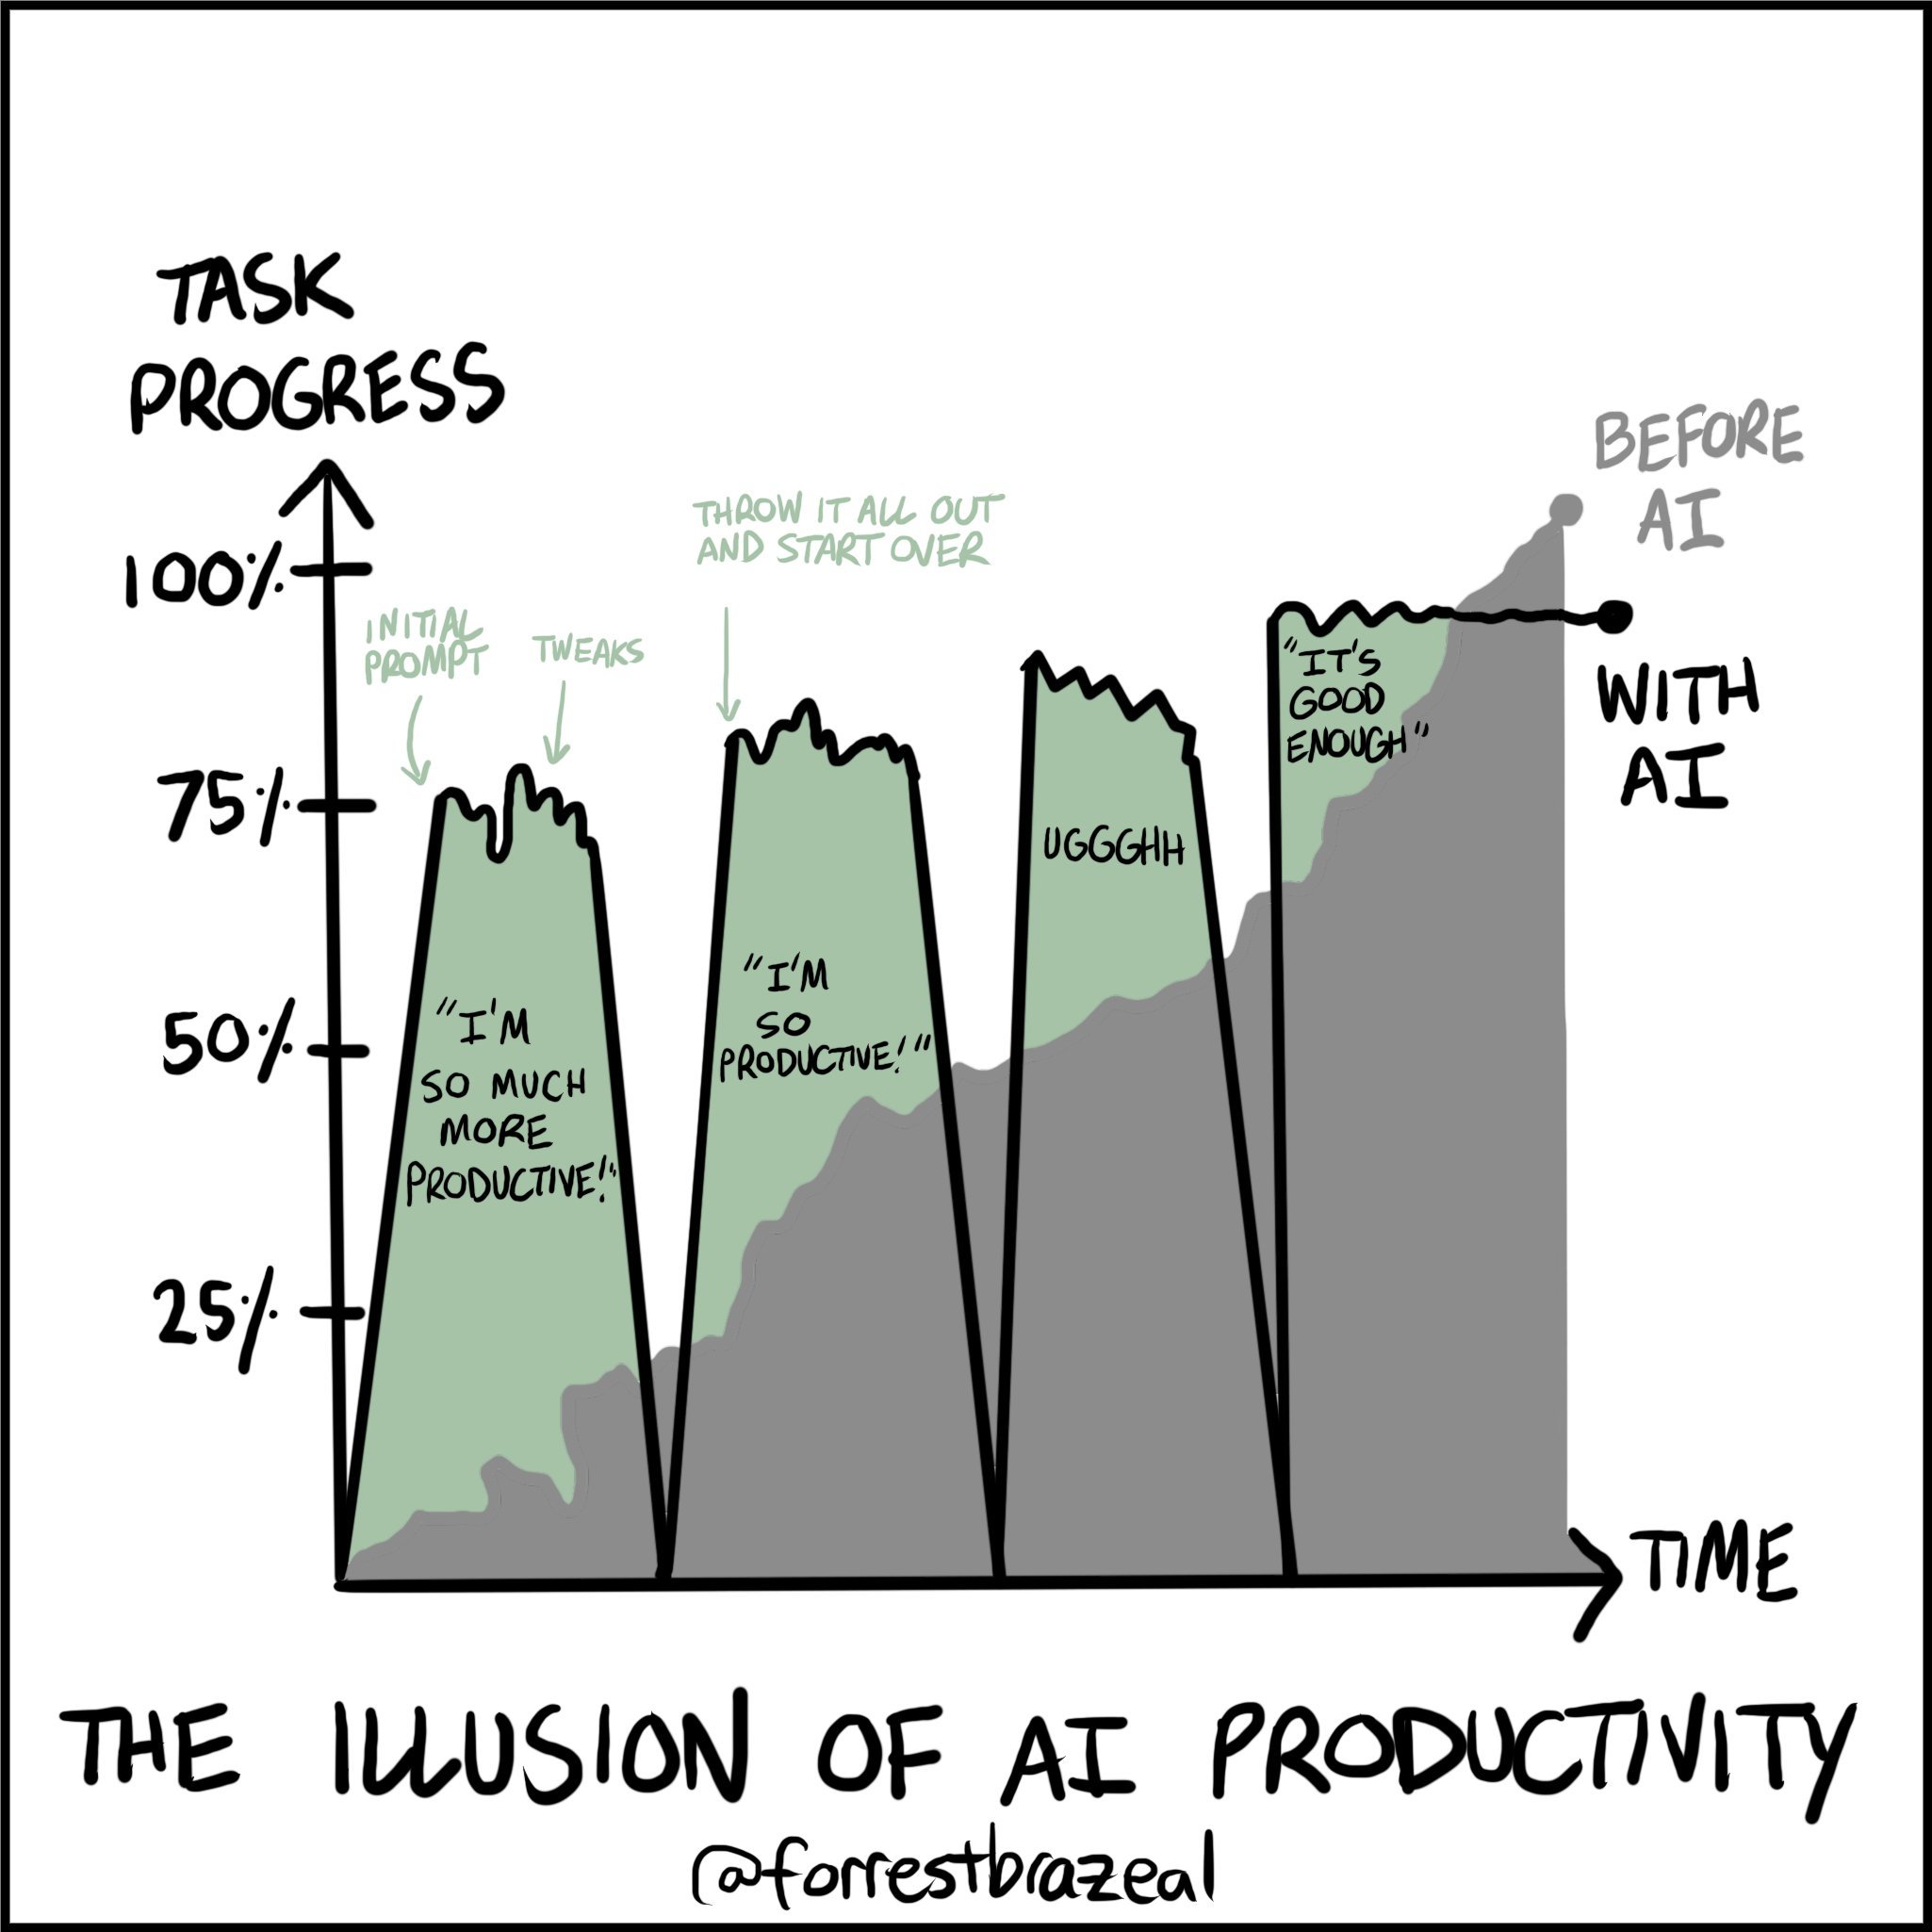
\includegraphics[width=.5\textwidth]{before_ai.jpeg} 
\end{frame}

\section{Introduction}
\begin{frame}[t]{Intelligent Software Engineering}
\begin{itemize}
\item \textbf{Beyond Traditional Methods}: AI and optimization techniques in software development
\item \textbf{Multiple Approaches}: Different intelligent methods for different problems
\item \textbf{Complementary Strengths}: Each method excels in specific domains
\item \textbf{Practical Applications}: Real-world tools and techniques used today
\item \textbf{Human-AI Collaboration}: Augmenting developer capabilities
\end{itemize}
\end{frame}

\section{Intelligent Methods Overview}
\begin{frame}[t]{Spectrum of Intelligent Approaches}
\begin{itemize}
\item \textbf{LLM-based Methods}: Natural language understanding and generation
\item \textbf{Search-based Optimization}: Evolutionary algorithms and local search
\item \textbf{Constraint Solving}: Formal methods and SAT solving
\item \textbf{Hybrid Approaches}: Combining multiple intelligent techniques
\item \textbf{Specialized AI}: Domain-specific machine learning models
\end{itemize}
\begin{figure}
\includegraphics[width=0.6\textwidth]{example-image}
\caption{Intelligent methods landscape in software engineering}
\end{figure}
\end{frame}

\section{Large Language Models (LLMs)}
\begin{frame}[t]{LLM-based Approaches}
\begin{itemize}
\item \textbf{Foundation}: Transformer architecture trained on massive text/code corpora
\item \textbf{Strengths}: Natural language understanding, code generation, documentation
\item \textbf{Applications}: Code completion, architecture design, API generation
\item \textbf{Examples}: GitHub Copilot, ChatGPT, CodeLlama
\item \textbf{Limitations}: Hallucinations, lack of formal guarantees
\end{itemize}
\end{frame}

\begin{frame}[fragile,t]{LLM Code Implementation Example}
\begin{verbatim}
// Prompt: "Implement a thread-safe LRU cache in Java"
public class LRUCache<K, V> {
    private final int capacity;
    private final LinkedHashMap<K, V> cache;
    
    public LRUCache(int capacity) {
        this.capacity = capacity;
        this.cache = new LinkedHashMap<K, V>(
            capacity, 0.75f, true) {
            protected boolean removeEldestEntry(
                Map.Entry<K, V> eldest) {
                return size() > capacity;
            }
        };
    }
    // Additional methods implemented by LLM...
}
\end{verbatim}
\end{frame}

\section{Search-Based Software Engineering}
\begin{frame}[t]{SBSE for Software Design and Implementation}
\begin{itemize}
\item \textbf{Foundation}: Treat software design as search problem in solution space
\item \textbf{Strengths}: Finding optimal or near-optimal design solutions
\item \textbf{Applications}: Algorithm selection, data structure optimization, code synthesis
\item \textbf{Key Insight}: Software design decisions can be optimized systematically
\end{itemize}
\end{frame}

\begin{frame}[t]{SBSE for Algorithm Selection and Implementation}
\begin{itemize}
\item \textbf{Problem}: Choose optimal algorithm for specific problem constraints
\item \textbf{Search Space}: Different algorithms and their parameterizations
\item \textbf{Fitness Function}: Runtime complexity, memory usage, implementation complexity
\item \textbf{Method}: Genetic algorithm exploring algorithm combinations
\item \textbf{Result}: Best algorithm choice with optimized parameters
\end{itemize}
\begin{figure}
\includegraphics[width=0.4\textwidth]{example-image}
\caption{Algorithm selection search space}
\end{figure}
\end{frame}

\begin{frame}[fragile,t]{SBSE for Data Structure Optimization}
\begin{verbatim}
// Problem: Optimize data structure for frequent insertions and rare lookups
// Search-based approach explores different data structure implementations

// Candidate solutions explored:
Solution 1: ArrayList with binary search (O(n) insert, O(log n) lookup)
Solution 2: LinkedList (O(1) insert, O(n) lookup)  
Solution 3: Balanced BST (O(log n) insert, O(log n) lookup)
Solution 4: Hash table with lazy deletion (O(1) insert, O(1) lookup)

// Fitness evaluation based on actual usage patterns
// Optimal solution selected: LinkedList for 90% insert-heavy workload
\end{verbatim}
\end{frame}

\begin{frame}[t]{SBSE for Code Synthesis and Completion}
\begin{itemize}
\item \textbf{Challenge}: Automatically complete partial code implementations
\item \textbf{Approach}: Genetic programming with code fragments as building blocks
\item \textbf{Fitness}: Type correctness, test case passing, code quality metrics
\item \textbf{Application}: Auto-completing complex algorithmic implementations
\item \textbf{Example}: Synthesizing efficient matrix operations from specifications
\end{itemize}
\end{frame}

\begin{frame}[fragile,t]{SBSE for API Implementation Completion}
\begin{verbatim}
// Partial implementation provided by developer
public interface DataProcessor {
    Data process(Input input);
    // Additional methods to be completed...
}

// SBSE generates complete implementation based on usage patterns
public class EfficientDataProcessor implements DataProcessor {
    public Data process(Input input) { /* optimized */ }
    public void validate(Data data) { /* auto-generated */ }
    public Result batchProcess(List<Input> inputs) { /* synthesized */ }
    // Additional methods synthesized by search-based approach
}
\end{verbatim}
\end{frame}

\section{Constraint-Based Methods}
\begin{frame}[t]{Constraint Solving for Software Design}
\begin{itemize}
\item \textbf{Foundation}: Encode design constraints as logical formulas
\item \textbf{Strengths}: Guaranteed satisfaction of specified properties
\item \textbf{Applications}: Type-driven synthesis, interface conformance, design patterns
\item \textbf{Key Benefit}: Formal verification of design decisions
\end{itemize}
\end{frame}

\begin{frame}[t]{Constraint-Based API Design and Implementation}
\begin{itemize}
\item \textbf{Problem}: Ensure API consistency and completeness
\item \textbf{Constraints}: Method preconditions, postconditions, invariants
\item \textbf{Method}: Enforce constraints during API evolution
\item \textbf{Application}: Automated checking of API design rules
\item \textbf{Benefit}: Early detection of design violations
\end{itemize}
\begin{figure}
\includegraphics[width=0.5\textwidth]{example-image}
\caption{Constraint-based API verification}
\end{figure}
\end{frame}

\begin{frame}[fragile,t]{Constraint-Based Code Completion}
\begin{verbatim}
// Partial code with type constraints
public <T> T process(List<T> items) {
    // Constraint solver infers missing operations
    // Constraints: T must support comparison, serialization
    // Based on usage context and method signatures
    
    // Solution generated by constraint solver:
    Collections.sort(items);  // T must implement Comparable
    return serializer.serialize(items); // T must be serializable
}

// Constraint solver ensures type safety and API consistency
\end{verbatim}
\end{frame}

\begin{frame}[t]{Constraint-Based Design Pattern Implementation}
\begin{itemize}
\item \textbf{Objective}: Correctly implement design patterns with formal guarantees
\item \textbf{Constraints}: Pattern-specific rules (Observer: subject-observer relationships)
\item \textbf{Method}: Encode pattern constraints as logical formulas
\item \textbf{Verification}: Check implementation against pattern constraints
\item \textbf{Completion}: Suggest missing pattern elements
\end{itemize}
\end{frame}

\begin{frame}[fragile,t]{Constraint-Based Singleton Pattern Enforcement}
\begin{verbatim}
// Constraint: Singleton class must have private constructor
// and static getInstance method

class DatabaseConnection {
    private static DatabaseConnection instance;
    
    // Constraint solver verifies:
    // ✓ Constructor is private
    // ✓ getInstance method exists and is static
    // ✓ Instance variable is static
    
    private DatabaseConnection() {}  // Verified: private
    public static DatabaseConnection getInstance() { // Verified: static
        if (instance == null) {
            instance = new DatabaseConnection();
        }
        return instance;
    }
}
\end{verbatim}
\end{frame}

\section{Natural Language Processing}
\begin{frame}[t]{NLP for Design Specification Processing}
\begin{itemize}
\item \textbf{Foundation}: Extract design intent from natural language
\item \textbf{Strengths}: Bridging requirement documents and implementation
\item \textbf{Applications}: Design pattern recognition, architecture extraction
\item \textbf{Evolution}: From manual analysis to automated understanding
\end{itemize}
\end{frame}

\section{Hybrid Approaches}
\begin{frame}[t]{Combining Methods for Design and Implementation}
\begin{itemize}
\item \textbf{LLM + Constraints}: Generate code with formal verification
\item \textbf{SBSE + Constraints}: Search with guaranteed constraint satisfaction
\item \textbf{NLP + SBSE}: Extract design constraints for optimization
\item \textbf{Multi-method Integration}: Comprehensive design assistance
\end{itemize}
\begin{figure}
\includegraphics[width=0.5\textwidth]{example-image}
\caption{Hybrid intelligent design system}
\end{figure}
\end{frame}

\begin{frame}[fragile,t]{Hybrid Example: Intelligent Code Completion}
\begin{verbatim}
// Developer writes partial method:
public String processData(String input) {
    // Step 1: LLM suggests initial completion
    if (input == null) return "";
    String result = input.trim();
    
    // Step 2: Constraint solver verifies null safety
    // ✓ input checked for null, ✓ return value not null
    
    // Step 3: SBSE optimizes string operations
    // Replaces inefficient concatenation with StringBuilder
    
    // Step 4: Final verified and optimized code
    StringBuilder sb = new StringBuilder();
    sb.append(result.toLowerCase());
    return sb.toString();
}
\end{verbatim}
\end{frame}

\section{Application Domains}
\begin{frame}[t]{Software Design and Implementation}
\begin{itemize}
\item \textbf{LLMs}: Rapid prototyping and boilerplate generation
\item \textbf{SBSE}: Optimal algorithm and data structure selection
\item \textbf{Constraint-based}: Type-safe API design and implementation
\item \textbf{Hybrid}: End-to-end design and implementation assistance
\end{itemize}
\end{frame}

\begin{frame}[t]{Code Completion and Synthesis}
\begin{itemize}
\item \textbf{LLMs}: Context-aware code suggestions
\item \textbf{SBSE}: Optimization-driven completion
\item \textbf{Constraint-based}: Type-directed synthesis with guarantees
\item \textbf{NLP}: Requirement-driven implementation
\end{itemize}
\end{frame}

\begin{frame}[t]{Architecture and Pattern Implementation}
\begin{itemize}
\item \textbf{Constraint-based}: Formal pattern verification
\item \textbf{SBSE}: Optimal pattern instantiation
\item \textbf{LLMs}: Pattern explanation and examples
\item \textbf{Hybrid}: Pattern-compliant architecture generation
\end{itemize}
\end{frame}

\section{Comparative Analysis}
\begin{frame}[t]{Method Comparison for Design/Implementation}
\begin{center}
\begin{tabular}{lccc}
\textbf{Method} & \textbf{Correctness Guarantees} & \textbf{Creativity} & \textbf{Speed} \\
\hline
LLM-based & Low & High & Fast \\
SBSE & Medium & Medium & Medium \\
Constraint-based & High & Low & Slow \\
Hybrid & High & High & Medium \\
\end{tabular}
\end{center}

\begin{itemize}
\item \textbf{Correctness Guarantees}: Formal verification capabilities
\item \textbf{Creativity}: Novel solution generation
\item \textbf{Speed}: Response time for practical use
\end{itemize}
\end{frame}

\begin{frame}[t]{Strengths for Design and Implementation}
\begin{itemize}
\item \textbf{LLMs}: Excellent for exploratory design and rapid prototyping
\item \textbf{SBSE}: Superior for optimization problems and algorithm selection
\item \textbf{Constraint-based}: Unmatched for correctness-critical components
\item \textbf{Hybrid}: Balanced approach for complex design challenges
\end{itemize}
\end{frame}

\section{Tools and Frameworks}
\begin{frame}[t]{Design and Implementation Tools}
\begin{itemize}
\item \textbf{LLM-based}: GitHub Copilot, Amazon CodeWhisperer, Tabnine
\item \textbf{SBSE}: Program synthesis tools (SKETCH, Rosette)
\item \textbf{Constraint-based}: Z3 for program verification, Alloy for design
\item \textbf{Hybrid}: Intelligent IDEs with multiple AI assistants
\end{itemize}
\end{frame}

\section{AI Pair Programming}

\begin{frame}[t]{What is AI Pair Programming?}
    \begin{block}{Definition}
        AI Pair Programming is a software development practice where developers collaborate with AI assistants to write code, receiving real-time suggestions, reviews, and optimizations.
    \end{block}
    
    \begin{columns}
        \begin{column}{0.6\textwidth}
            \textbf{Key Characteristics:}
            \begin{itemize}
                \item \textbf{Real-time Collaboration}: AI provides instant code suggestions
                \item \textbf{Knowledge Sharing}: AI transfers best practices and patterns
                \item \textbf{Quality Assurance}: Immediate code review and optimization
                \item \textbf{Learning Acceleration}: Opportunity for beginners to learn from experts
            \end{itemize}
        \end{column}
        \begin{column}{0.4\textwidth}
            \centering
            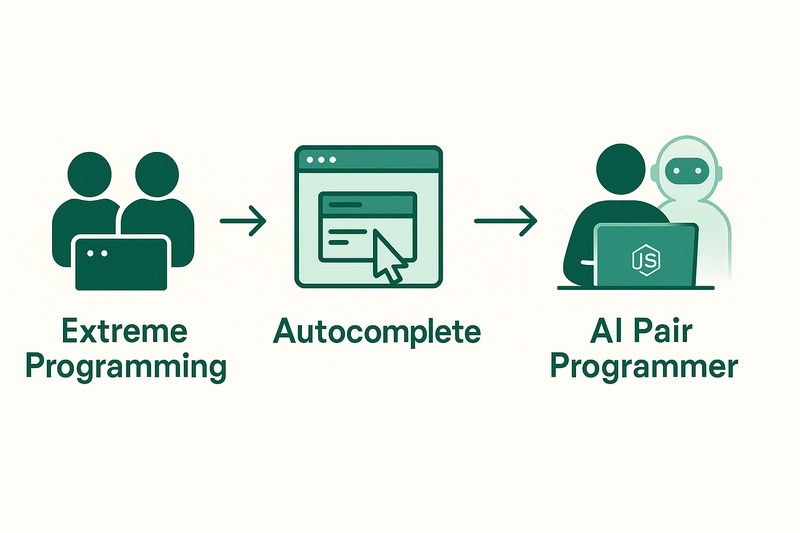
\includegraphics[width=0.9\textwidth]{images/ai-pair-programming.png}
            % \captionof{figure}{AI Pair Programming Concept}
        \end{column}
    \end{columns}
\end{frame}

\begin{frame}[t]{Traditional vs. AI Pair Programming}
    \begin{table}
        \centering
        \begin{tabular}{p{0.3\textwidth}|p{0.3\textwidth}|p{0.3\textwidth}}
            \textbf{Aspect} & \textbf{Traditional} & \textbf{AI Pair Programming} \\
            \hline
            Availability & Requires another developer & Available 24/7 \\
            Knowledge & Limited to developers' experience & Vast best practices coverage \\
            Consistency & Varies by individuals & Highly consistent standards \\
            Cost & Two developers' time & Lower tool costs \\
            Learning & Bidirectional knowledge transfer & Primarily learning from AI \\
            Creativity & Mutual brainstorming & Pattern-based suggestions \\
        \end{tabular}
        \caption{Comparison of Pair Programming Approaches}
    \end{table}
\end{frame}

\begin{frame}[t]{Popular AI Pair Programming Tools}
    \begin{columns}
        \begin{column}{0.5\textwidth}
            \textbf{IDE-Integrated Tools:}
            \begin{itemize}
                \item \textbf{GitHub Copilot}
                \begin{itemize}
                    \item Most popular AI programming assistant
                    \item Multi-language support
                    \item Context-aware code generation
                \end{itemize}
                
                \item \textbf{Amazon CodeWhisperer}
                \begin{itemize}
                    \item AWS-optimized integration
                    \item Security scanning features
                    \item Free for individual use
                \end{itemize}
            \end{itemize}
        \end{column}
        \begin{column}{0.5\textwidth}
            \textbf{Other Tools:}
            \begin{itemize}
                \item \textbf{Tabnine}
                \begin{itemize}
                    \item On-premise deployment options
                    \item Privacy-focused
                \end{itemize}
                
                \item \textbf{Cursor}
                \begin{itemize}
                    \item AI-first code editor
                    \item Deep code understanding
                \end{itemize}
                
                \item \textbf{Replit AI}
                \begin{itemize}
                    \item Cloud development environment
                    \item Real-time collaboration
                \end{itemize}
            \end{itemize}
        \end{column}
    \end{columns}
\end{frame}

\begin{frame}[t,fragile]{AI Pair Programming Workflow}
    \begin{lstlisting}[style=code, caption={Typical AI Pair Programming Interaction}]
// Developer: Write function signature
function calculateTax(income: number, deductions: number): number {
    // Developer: Add comment describing requirements
    // Calculate tax based on income and deductions
    // Use progressive tax brackets
    
    // AI Assistant: Auto-generates implementation
    const taxableIncome = income - deductions;
    
    if (taxableIncome <= 0) return 0;
    
    const brackets = [
        { limit: 10000, rate: 0.1 },
        { limit: 40000, rate: 0.2 },
        { limit: Infinity, rate: 0.3 }
    ];
    
    let tax = 0;
    let previousLimit = 0;
    
    for (const bracket of brackets) {
        if (taxableIncome > previousLimit) {
            const amountInBracket = Math.min(
                taxableIncome - previousLimit, 
                bracket.limit - previousLimit
            );
            tax += amountInBracket * bracket.rate;
            previousLimit = bracket.limit;
        }
    }
    
    return tax;
}
    \end{lstlisting}
\end{frame}

\begin{frame}[t]{AI Pair Programming in Requirements Engineering}
    \begin{block}{Bridging Requirements and Code}
        AI Pair Programming helps transform requirements specifications directly into executable code
    \end{block}
    
    \textbf{Specific Applications:}
    \begin{itemize}
        \item \textbf{Requirements Prototyping}: Quick conversion of requirements to working prototypes
        \item \textbf{Specification Validation}: Verify requirement feasibility through code
        \item \textbf{Test Case Generation}: Auto-generate test code from requirements
        \item \textbf{API Design}: Generate code frameworks from interface requirements
        \item \textbf{Database Design}: Convert data requirements to SQL schemas
    \end{itemize}
    
    \begin{exampleblock}{Example Workflow}
        Requirements Document → AI Understanding → Code Framework → Iterative Refinement → Final Implementation
    \end{exampleblock}
\end{frame}

\begin{frame}[t,fragile]{Requirements-to-Code Transformation Example}
    \begin{columns}
        \begin{column}{0.5\textwidth}
            \textbf{Requirements Specification:}
            \begin{lstlisting}[style=code]
User Requirements:
- User registration
- Email verification
- Password strength check
- Welcome email sending

Business Rules:
- Password minimum 8 chars
- Mixed case and numbers
- Unique email required
- Verification code valid 10min
            \end{lstlisting}
        \end{column}
        \begin{column}{0.5\textwidth}
            \textbf{AI-Generated Code Framework:}
            \begin{lstlisting}[style=code]
// User registration service
class UserService {
    async register(userData) {
        // Validate email uniqueness
        // Check password strength
        // Create user record
        // Send verification email
        // Return success response
    }
    
    isStrongPassword(password) {
        // Check length >= 8
        // Check uppercase/lowercase
        // Check contains number
    }
}
            \end{lstlisting}
        \end{column}
    \end{columns}
\end{frame}

\begin{frame}[t]{Best Practices for Students}
    \begin{columns}
        \begin{column}{0.5\textwidth}
            \textbf{Effective Patterns:}
            \begin{enumerate}
                \item \textbf{Clear Intent}: Write descriptive comments
                \item \textbf{Incremental Development}: Small steps, frequent validation
                \item \textbf{Code Review}: Critically evaluate AI suggestions
                \item \textbf{Test-Driven}: Write tests first, then generate code
                \item \textbf{Security First}: Validate security and edge cases
            \end{enumerate}
        \end{column}
        \begin{column}{0.5\textwidth}
            \textbf{Pitfalls to Avoid:}
            \begin{itemize}
                \item \textbf{Blind Acceptance}: Not reviewing AI-generated code
                \item \textbf{Over-reliance}: Losing programming thinking skills
                \item \textbf{Security Risks}: Ignoring security reviews
                \item \textbf{Copyright Issues}: Using protected code
                \item \textbf{Performance Neglect}: Skipping performance testing
            \end{itemize}
        \end{column}
    \end{columns}
    
    \vspace{0.5cm}
    \textbf{Quality Assurance Process:}
    \begin{enumerate}
        \item AI suggests code → 2. Student reviews → 3. Run tests → 4. Integrate to codebase
    \end{enumerate}
\end{frame}

\begin{frame}[t,fragile]{Test-Driven AI Pair Programming}
    \begin{block}{Test-First Development}
        Write test cases first, then use AI to generate implementation code that passes the tests
    \end{block}
    
    \begin{columns}
        \begin{column}{0.5\textwidth}
            \textbf{Test Cases Example:}
            \begin{lstlisting}[style=code]
// Write tests first
describe('Tax Calculator', () => {
    test('calculates tax correctly', () => {
        expect(calculateTax(50000, 5000))
            .toBe(8500);
    });
    
    test('handles zero income', () => {
        expect(calculateTax(0, 1000))
            .toBe(0);
    });
});
            \end{lstlisting}
        \end{column}
        \begin{column}{0.5\textwidth}
            \textbf{AI Generates Implementation:}
            \begin{lstlisting}[style=code]
// AI implements based on tests
function calculateTax(income, deductions) {
    // Implementation logic...
    // Must pass all test cases
}
            \end{lstlisting}
        \end{column}
    \end{columns}
    
    \textbf{Benefits for Learning:}
    \begin{itemize}
        \item Ensures code meets requirements
        \item Automatic validation of correctness
        \item Facilitates regression testing
        \item Improves code quality awareness
    \end{itemize}
\end{frame}

\begin{frame}[t,fragile]{Effective Prompt Engineering for Students}
    \begin{lstlisting}[style=code, caption={Structured Prompt Template}]
// Poor prompt:
"write a sorting function"

// Effective prompt:
"""
Act as an experienced JavaScript developer. 
Help me implement a quicksort function.

Requirements:
- Function name: quickSort
- Parameters: array (numbers)
- Returns: new sorted array
- Use recursive implementation with comments

Example input: [3, 1, 4, 1, 5, 9, 2, 6]
Expected output: [1, 1, 2, 3, 4, 5, 6, 9]

Please explain the algorithm approach first, 
then provide the code implementation.
"""
    \end{lstlisting}
    
    \textbf{Prompt Engineering Tips:}
    \begin{itemize}
        \item Specify role and context clearly
        \item Include specific technical requirements
        \item Provide input/output examples
        \item Define code standards and constraints
        \item Request step-by-step explanations
    \end{itemize}
\end{frame}

\begin{frame}[t]{Learning Benefits for Students}
    \begin{columns}
        \begin{column}{0.5\textwidth}
            \textbf{Technical Skills:}
            \begin{itemize}
                \item \textbf{Faster Learning}: 2-3x acceleration in skill acquisition
                \item \textbf{Best Practices}: Exposure to professional coding standards
                \item \textbf{Pattern Recognition}: Learn common algorithms and patterns
                \item \textbf{Debugging Skills}: See how AI approaches problem-solving
                \item \textbf{Code Quality}: Understand what makes code maintainable
            \end{itemize}
        \end{column}
        \begin{column}{0.5\textwidth}
            \textbf{Professional Development:}
            \begin{itemize}
                \item \textbf{Confidence Building}: Quick success with complex tasks
                \item \textbf{Portfolio Growth}: Ability to complete more projects
                \item \textbf{Industry Preparation}: Learn tools used in professional environments
                \item \textbf{Collaboration Skills}: Practice code review and collaboration
                \item \textbf{Problem Decomposition}: Learn to break down complex problems
            \end{itemize}
        \end{column}
    \end{columns}
\end{frame}

\begin{frame}[t]{Common Challenges for Student Developers}
    \begin{columns}
        \begin{column}{0.5\textwidth}
            \textbf{Technical Challenges:}
            \begin{itemize}
                \item \textbf{Understanding Limitations}: When AI suggestions are wrong
                \item \textbf{Over-complex Solutions}: AI may suggest advanced patterns
                \item \textbf{Dependency Management}: Handling library recommendations
                \item \textbf{Debugging AI Code}: Tracing issues in generated code
                \item \textbf{Performance Awareness}: Recognizing inefficient solutions
            \end{itemize}
        \end{column}
        \begin{column}{0.5\textwidth}
            \textbf{Learning Challenges:}
            \begin{itemize}
                \item \textbf{Skill Dependency}: Risk of relying too much on AI
                \item \textbf{Conceptual Gaps}: Missing fundamental understanding
                \item \textbf{Critical Thinking}: Need to evaluate AI suggestions
                \item \textbf{Academic Integrity}: Proper use in coursework
                \item \textbf{Balance Finding}: When to use AI vs. manual coding
            \end{itemize}
        \end{column}
    \end{columns}
    
    \vspace{0.5cm}
    \textbf{Strategies for Success:}
    \begin{itemize}
        \item Use AI for learning, not just completing assignments
        \item Always review and understand AI-generated code
        \item Practice manual coding regularly
        \item Discuss AI suggestions with instructors
        \item Document what you learn from each interaction
    \end{itemize}
\end{frame}

\begin{frame}[t]{Academic Integrity Considerations}
    \begin{block}{Responsible Use in Education}
        AI Pair Programming should enhance learning, not replace it
    \end{block}
    
    \textbf{Institutional Guidelines:}
    \begin{itemize}
        \item \textbf{Check Course Policies}: Understand what's allowed in each course
        \item \textbf{Transparency}: Disclose AI assistance in submissions
        \item \textbf{Learning Focus}: Use AI to understand, not just complete work
        \item \textbf{Proper Attribution}: Credit AI contributions appropriately
    \end{itemize}
    
    \textbf{Recommended Practices:}
    \begin{itemize}
        \item Use AI for learning concepts, not assignment completion
        \item Document your learning process with AI
        \item Show both AI suggestions and your modifications
        \item Discuss AI interactions in code comments
        \item Focus on understanding the underlying concepts
    \end{itemize}
    
    \begin{alertblock}{Important}
        Always follow your institution's academic integrity policies regarding AI tool usage
    \end{alertblock}
\end{frame}

\begin{frame}[t]{Practical Exercise: Student Project Workflow}
    \textbf{Step-by-Step Learning Approach:}
    
    \begin{enumerate}
        \item \textbf{Requirements Analysis}: Use AI to understand project requirements
        \item \textbf{Design Phase}: Get AI suggestions for architecture and patterns
        \item \textbf{Implementation}: Use AI for code generation with active learning
        \item \textbf{Testing}: Generate test cases and learn testing strategies
        \item \textbf{Review}: Use AI for code review and optimization suggestions
        \item \textbf{Reflection}: Document what you learned from the AI interactions
    \end{enumerate}
    
    \textbf{Learning Objectives:}
    \begin{itemize}
        \item Understand how to translate requirements to code
        \item Learn professional coding standards and patterns
        \item Develop critical evaluation skills for code quality
        \item Practice iterative development and refinement
        \item Build confidence in tackling complex programming tasks
    \end{itemize}
\end{frame}

\begin{frame}[t,fragile]{Sample Student Project: Todo List Application}
    \begin{columns}
        \begin{column}{0.5\textwidth}
            \textbf{Requirements:}
            \begin{lstlisting}[style=code]
Create a todo list app with:
- Add new tasks
- Mark tasks complete
- Delete tasks
- Filter tasks (all/active/completed)
- Local storage persistence
- Responsive design
            \end{lstlisting}
        \end{column}
        \begin{column}{0.5\textwidth}
            \textbf{AI-Assisted Learning:}
            \begin{itemize}
                \item Get HTML/CSS structure suggestions
                \item Learn JavaScript event handling
                \item Understand local storage API
                \item Study responsive design patterns
                \item Practice code organization
            \end{itemize}
        \end{column}
    \end{columns}
    
    \vspace{0.5cm}
    \textbf{Learning Outcomes:}
    \begin{itemize}
        \item DOM manipulation techniques
        \item State management patterns
        \item Data persistence methods
        \item UI/UX design considerations
        \item Problem decomposition skills
    \end{itemize}
\end{frame}

\begin{frame}[t]{Future Career Preparation}
    \begin{block}{Industry Relevance}
        AI Pair Programming skills are increasingly valuable in professional software development
    \end{block}
    
    \textbf{Career Benefits:}
    \begin{itemize}
        \item \textbf{Technical Adaptability}: Experience with modern development tools
        \item \textbf{Efficiency Skills}: Ability to work effectively with AI assistants
        \item \textbf{Quality Mindset}: Understanding of code quality standards
        \item \textbf{Collaboration Experience}: Practice with AI-human teamwork
        \item \textbf{Continuous Learning}: Comfort with evolving technology tools
    \end{itemize}
    
    \textbf{Industry Trends:}
    \begin{itemize}
        \item AI assistance becoming standard in development environments
        \item Growing demand for developers who can work effectively with AI
        \item Increased focus on code quality and maintainability
        \item Emphasis on rapid prototyping and iteration
        \item Importance of clear communication and requirements understanding
    \end{itemize}
\end{frame}

\begin{frame}[t]{Getting Started: Student Action Plan}
    \textbf{Immediate Steps:}
    \begin{enumerate}
        \item \textbf{Choose a Tool}: Start with GitHub Copilot (student discount available)
        \item \textbf{Small Projects}: Begin with simple coding exercises
        \item \textbf{Active Learning}: Always understand the code AI generates
        \item \textbf{Document Learning}: Keep notes on patterns and techniques learned
        \item \textbf{Seek Feedback}: Discuss AI interactions with instructors and peers
    \end{enumerate}
    
    \textbf{Learning Resources:}
    \begin{itemize}
        \item GitHub Education Pack (free access to developer tools)
        \item Online tutorials on effective prompt engineering
        \item University coding clubs and workshops
        \item Open source projects for practice
        \item Peer programming sessions with AI discussion
    \end{itemize}
    
    \begin{exampleblock}{Call to Action}
        Start experimenting with AI Pair Programming in your next coding project! Focus on using it as a learning tool to enhance your understanding, not just complete assignments.
    \end{exampleblock}
\end{frame}

\begin{frame}[t]{Summary: AI as Learning Partner}
    \begin{columns}
        \begin{column}{0.6\textwidth}
            \textbf{Key Takeaways:}
            \begin{itemize}
                \item AI Pair Programming accelerates learning when used intentionally
                \item Critical thinking and code review skills remain essential
                \item Balance AI assistance with fundamental skill development
                \item Focus on understanding concepts, not just completing work
                \item Document and reflect on your learning journey
            \end{itemize}
        \end{column}
        \begin{column}{0.4\textwidth}
            \centering
            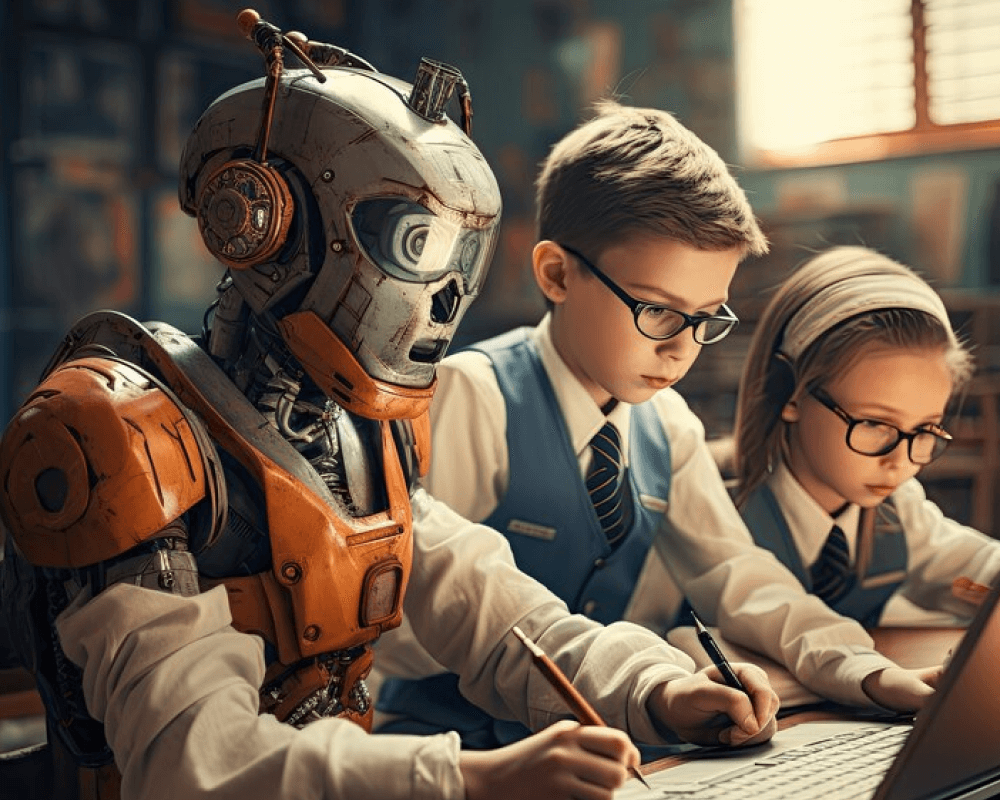
\includegraphics[width=0.9\textwidth]{images/ai-learning-partner.png}
            % \captionof{figure}{AI as Learning Enhancement}
        \end{column}
    \end{columns}
    
    \vspace{0.5cm}
    \begin{block}{Successful Approach}
        The most effective students use AI as a tutor and collaborator, not a crutch. They maintain active engagement, ask questions, and focus on deep understanding.
    \end{block}
\end{frame}

\section{How AI-Assisted Programming Works Under the Hood}

\begin{frame}[t]{Overview of AI-Assisted Programming Architecture}
    \begin{block}{High-Level System Architecture}
        AI-assisted programming systems combine several AI technologies to understand, generate, and manipulate code.
    \end{block}
    
    \begin{columns}[t]
        \begin{column}{0.6\textwidth}
            \textbf{Core Components:}
            \begin{itemize}
                \item \textbf{Language Models}: Understand and generate code
                \item \textbf{Tokenization}: Convert code to machine-readable format
                \item \textbf{Training Data}: Massive code repositories and documentation
                \item \textbf{Context Management}: Handle large codebases and dependencies
                \item \textbf{Code Analysis}: Static analysis and pattern recognition
            \end{itemize}
        \end{column}
        \begin{column}{0.4\textwidth}
            \centering
            \includegraphics[width=0.9\textwidth]{example-image} % {images/ai-architecture-overview.png}
            % \captionof{figure}{System Architecture}
        \end{column}
    \end{columns}
\end{frame}

\begin{frame}[t]{The Training Process: How Models Learn Code}
    \begin{block}{Pre-training on Massive Code Corpora}
        Models are trained on billions of lines of code from various sources:
    \end{block}
    
    \begin{columns}[t]
        \begin{column}{0.5\textwidth}
            \textbf{Training Data Sources:}
            \begin{itemize}
                \item GitHub repositories (public)
                \item Stack Overflow questions/answers
                \item Documentation and tutorials
                \item Code competition solutions
                \item Open source libraries
            \end{itemize}
        \end{column}
        \begin{column}{0.5\textwidth}
            \textbf{Learning Objectives:}
            \begin{itemize}
                \item Syntax and grammar patterns
                \item API usage patterns
                \item Common algorithms and data structures
                \item Code commenting styles
                \item Error handling patterns
            \end{itemize}
        \end{column}
    \end{columns}
    
    \vspace{0.3cm}
    \begin{alertblock}{Important}
        Models learn statistical patterns, not true understanding. They predict what comes next based on training data.
    \end{alertblock}
\end{frame}

\begin{frame}[t]{Tokenization: Converting Code to Numbers}
    \begin{block}{Code Tokenization Process}
        Code is broken down into tokens (meaningful units) before processing.
    \end{block}
    
    \begin{exampleblock}{Example: Python Function}
        \texttt{def calculate\_sum(a, b):\ return a + b}
    \end{exampleblock}
    
    \textbf{Tokenization Result:}
    \begin{itemize}
        \item \texttt{["def", "calculate\_sum", "(", "a", ",", "b", ")", ":", "return", "a", "+", "b"]}
    \end{itemize}
    
    \begin{columns}[t]
        \begin{column}{0.5\textwidth}
            \textbf{Specialized Tokenizers:}
            \begin{itemize}
                \item \textbf{WordPiece}: Used by Codex/Copilot
                \item \textbf{Byte Pair Encoding (BPE)}: Common in GPT models
                \item \textbf{SentencePiece}: Google's approach
            \end{itemize}
        \end{column}
        \begin{column}{0.5\textwidth}
            \textbf{Token Types:}
            \begin{itemize}
                \item Keywords (\texttt{def}, \texttt{return})
                \item Identifiers (\texttt{calculate\_sum})
                \item Operators (\texttt{+}, \texttt{=})
                \item Literals (numbers, strings)
                \item Punctuation
            \end{itemize}
        \end{column}
    \end{columns}
\end{frame}

\begin{frame}[t,fragile]{Transformer Architecture: The Brain Behind Code Generation}
    \begin{block}{Transformer Neural Networks}
        Most code generation models use transformer architecture with attention mechanisms.
    \end{block}
    
    \begin{lstlisting}[style=code, basicstyle=\ttfamily\tiny]
# Simplified transformer architecture for code generation
class CodeTransformer:
    def __init__(self):
        self.embedding_layer = Embedding(vocab_size, hidden_size)
        self.attention_layers = MultiHeadAttention(num_heads, hidden_size)
        self.feed_forward = FeedForward(hidden_size)
        self.output_layer = Linear(hidden_size, vocab_size)
    
    def generate_code(self, prompt_tokens):
        # Convert tokens to embeddings
        embeddings = self.embedding_layer(prompt_tokens)
        
        # Process through multiple attention layers
        for layer in self.attention_layers:
            embeddings = layer(embeddings)
        
        # Generate probability distribution for next token
        logits = self.output_layer(embeddings)
        next_token_probs = softmax(logits)
        
        return next_token_probs
    \end{lstlisting}
    
    \textbf{Key Components:}
    \begin{itemize}
        \item \textbf{Self-Attention}: Weights importance of different tokens
        \item \textbf{Multi-Head Attention}: Multiple attention mechanisms in parallel
        \item \textbf{Positional Encoding}: Maintains token order information
    \end{itemize}
\end{frame}

\begin{frame}[t]{Attention Mechanism: Understanding Code Context}
    \begin{block}{How Attention Works}
        Attention mechanisms allow the model to focus on relevant parts of the code context.
    \end{block}
    
    \begin{columns}[t]
        \begin{column}{0.6\textwidth}
            \textbf{Attention Process:}
            \begin{enumerate}
                \item Convert tokens to Query, Key, Value vectors
                \item Compute attention scores (similarity between Query and Key)
                \item Apply softmax to get attention weights
                \item Weighted sum of Value vectors
            \end{enumerate}
            
            \textbf{Mathematical Formula:}
            \[
            \text{Attention}(Q, K, V) = \text{softmax}\left(\frac{QK^T}{\sqrt{d_k}}\right)V
            \]
        \end{column}
        \begin{column}{0.4\textwidth}
            \centering
            \includegraphics[width=0.9\textwidth]{example-image} %{images/attention-mechanism.png}
            % \captionof{figure}{Attention Weights Visualization}
        \end{column}
    \end{columns}
    
    \textbf{Example:} When generating a function call, attention focuses on the function definition and relevant variables.
\end{frame}

\begin{frame}[t,fragile]{Code Representation: Abstract Syntax Trees (ASTs)}
    \begin{block}{Structured Code Representation}
        Models often use ASTs to understand code structure beyond plain text.
    \end{block}
    
    \begin{columns}[t]
        \begin{column}{0.5\textwidth}
            \textbf{Simple Python Code:}
            \begin{lstlisting}[style=code, basicstyle=\ttfamily\scriptsize]
def factorial(n):
    if n <= 1:
        return 1
    else:
        return n * factorial(n-1)
            \end{lstlisting}
        \end{column}
        \begin{column}{0.5\textwidth}
            \textbf{AST Structure:}
            \begin{itemize}
                \item FunctionDef: factorial
                \begin{itemize}
                    \item Arguments: n
                    \item Body:
                    \begin{itemize}
                        \item If: n <= 1
                        \item Return: 1
                        \item Else: Return n * factorial(n-1)
                    \end{itemize}
                \end{itemize}
            \end{itemize}
        \end{column}
    \end{columns}
    
    \vspace{0.3cm}
    \textbf{Benefits of AST-based Approaches:}
    \begin{itemize}
        \item Better understanding of code structure
        \item Improved syntax correctness
        \item Easier code transformation
        \item Better error detection
    \end{itemize}
\end{frame}

\begin{frame}[t]{Training Objectives: How Models Learn to Code}
    \begin{block}{Different Learning Approaches}
        Models use various training objectives to learn coding patterns.
    \end{block}
    
    \begin{columns}[t]
        \begin{column}{0.5\textwidth}
            \textbf{Pre-training Objectives:}
            \begin{itemize}
                \item \textbf{Masked Language Modeling}: Predict masked tokens
                \item \textbf{Causal Language Modeling}: Predict next token
                \item \textbf{Denoising Autoencoding}: Reconstruct corrupted code
                \item \textbf{Code Translation}: Convert between languages/styles
            \end{itemize}
        \end{column}
        \begin{column}{0.5\textwidth}
            \textbf{Fine-tuning Objectives:}
            \begin{itemize}
                \item \textbf{Code Completion}: Complete partial code
                \item \textbf{Bug Fixing}: Identify and fix errors
                \item \textbf{Documentation Generation}: Write comments from code
                \item \textbf{Test Generation}: Create tests from function signatures
            \end{itemize}
        \end{column}
    \end{columns}
    
    \vspace{0.3cm}
    \begin{exampleblock}{Masked Language Modeling Example}
        Input: \texttt{def factorial(n): if n <= 1: return [MASK] else: return n * factorial(n-1)} \\
        Model learns to predict: \texttt{1}
    \end{exampleblock}
\end{frame}

\begin{frame}[t]{Context Window Management}
    \begin{block}{Handling Large Codebases}
        Models need to manage context efficiently due to limited input size.
    \end{block}
    
    \textbf{Context Window Challenges:}
    \begin{itemize}
        \item Typical limits: 2K-128K tokens
        \item Large files exceed these limits
        \item Need to maintain relevant context
    \end{itemize}
    
    \begin{columns}[t]
        \begin{column}{0.5\textwidth}
            \textbf{Context Selection Strategies:}
            \begin{itemize}
                \item \textbf{Sliding Window}: Recent tokens + some history
                \item \textbf{Hierarchical Attention}: Focus on important sections
                \item \textbf{Code Chunking}: Break large files into logical units
                \item \textbf{Import Analysis}: Prioritize imported/used components
            \end{itemize}
        \end{column}
        \begin{column}{0.5\textwidth}
            \textbf{Advanced Techniques:}
            \begin{itemize}
                \item \textbf{Long-range Attention}: Sparse attention mechanisms
                \item \textbf{Memory Networks}: External memory for large context
                \item \textbf{Graph Neural Networks}: Represent code dependencies
                \item \textbf{Retrieval-Augmented Generation}: Retrieve relevant context
            \end{itemize}
        \end{column}
    \end{columns}
\end{frame}

\begin{frame}[t]{Code Embeddings: Representing Code Semantically}
    \begin{block}{Learning Code Representations}
        Models create dense vector representations that capture code semantics.
    \end{block}
    
    \textbf{Embedding Techniques:}
    \begin{itemize}
        \item \textbf{Token Embeddings}: Represent individual tokens
        \item \textbf{Positional Embeddings}: Encode token positions
        \item \textbf{Type Embeddings}: Distinguish tokens by type (keyword, variable, etc.)
        \item \textbf{Contextual Embeddings}: Vary based on surrounding context
    \end{itemize}
    
    \begin{columns}[t]
        \begin{column}{0.6\textwidth}
            \textbf{Semantic Code Similarity:}
            \begin{itemize}
                \item Similar code snippets have similar embeddings
                \item Enables code search and recommendation
                \item Helps with code completion and bug detection
            \end{itemize}
            
            \textbf{Example:}
            \texttt{for i in range(10):} and \texttt{for j in range(10):} have similar embeddings despite different variable names.
        \end{column}
        \begin{column}{0.4\textwidth}
            \centering
            \includegraphics[width=0.9\textwidth]{example-image} % {images/code-embeddings.png}
            % \captionof{figure}{Code Embedding Space}
        \end{column}
    \end{columns}
\end{frame}

\begin{frame}[t]{Fine-Tuning for Specific Tasks}
    \begin{block}{Specializing General Models}
        Pre-trained models are fine-tuned for specific programming tasks.
    \end{block}
    
    \textbf{Common Fine-Tuning Approaches:}
    \begin{itemize}
        \item \textbf{Task-Specific Datasets}: Curated examples for specific tasks
        \item \textbf{Instruction Tuning}: Teach models to follow programming instructions
        \item \textbf{Reinforcement Learning}: Optimize for code quality metrics
        \item \textbf{Multi-task Learning}: Learn multiple programming tasks simultaneously
    \end{itemize}
    
    \begin{columns}[t]
        \begin{column}{0.5\textwidth}
            \textbf{Fine-Tuning Data Examples:}
            \begin{itemize}
                \item Code completion pairs
                \item Bug-fix examples
                \item Documentation-code pairs
                \item Test-case implementations
            \end{itemize}
        \end{column}
        \begin{column}{0.5\textwidth}
            \textbf{Optimization Objectives:}
            \begin{itemize}
                \item Code compilation success rate
                \item Test case pass rate
                \item Code quality metrics
                \item Human preference alignment
            \end{itemize}
        \end{column}
    \end{columns}
\end{frame}

\begin{frame}[t,fragile]{Code Generation Process: Step by Step}
    \begin{block}{Autoregressive Generation}
        Models generate code one token at a time, conditioning on previous tokens.
    \end{block}
    
    \begin{lstlisting}[style=code, basicstyle=\ttfamily\tiny]
function generate_code(prompt, max_length=100):
    tokens = tokenize(prompt)
    generated_tokens = []
    
    for i in range(max_length):
        # Get model predictions for next token
        logits = model.predict(tokens + generated_tokens)
        
        # Apply sampling strategy
        next_token = sample_from_logits(logits)
        
        # Stop if end-of-code token generated
        if next_token == EOS_TOKEN:
            break
            
        generated_tokens.append(next_token)
    
    return detokenize(generated_tokens)

function sample_from_logits(logits):
    # Various sampling strategies:
    # 1. Greedy: argmax(logits)
    # 2. Temperature sampling: softmax(logits / temperature)
    # 3. Top-k sampling: sample from top k tokens
    # 4. Nucleus sampling: sample from top p cumulative probability
    return implementation_choice(logits)
    \end{lstlisting}
\end{frame}

\begin{frame}[t]{Sampling Strategies for Code Generation}
    \begin{block}{Balancing Creativity and Correctness}
        Different sampling strategies produce different types of code suggestions.
    \end{block}
    
    \begin{columns}[t]
        \begin{column}{0.5\textwidth}
            \textbf{Common Strategies:}
            \begin{itemize}
                \item \textbf{Greedy Sampling}: Always choose most likely token
                \begin{itemize}
                    \item Pros: Deterministic, fast
                    \item Cons: Can get stuck in loops
                \end{itemize}
                
                \item \textbf{Temperature Sampling}: Control randomness
                \begin{itemize}
                    \item Low temp: More deterministic
                    \item High temp: More creative
                \end{itemize}
            \end{itemize}
        \end{column}
        \begin{column}{0.5\textwidth}
            \textbf{Advanced Strategies:}
            \begin{itemize}
                \item \textbf{Top-k Sampling}: Sample from k most likely tokens
                \item \textbf{Nucleus Sampling}: Sample from tokens covering probability mass p
                \item \textbf{Beam Search}: Keep multiple candidate sequences
                \item \textbf{Constrained Decoding}: Enforce syntax constraints
            \end{itemize}
        \end{column}
    \end{columns}
    
    \vspace{0.3cm}
    \textbf{Code-Specific Considerations:}
    \begin{itemize}
        \item Syntax constraints must be respected
        \item Variable name consistency matters
        \item API usage patterns should be correct
        \item Code style consistency is important
    \end{itemize}
\end{frame}

\begin{frame}[t]{Error Handling and Code Correctness}
    \begin{block}{Ensuring Generated Code Works}
        Systems incorporate multiple mechanisms to improve code quality.
    \end{block}
    
    \textbf{Error Detection Mechanisms:}
    \begin{itemize}
        \item \textbf{Syntax Checking}: Ensure generated code parses correctly
        \item \textbf{Type Inference}: Check type consistency
        \item \textbf{Static Analysis}: Detect common errors and anti-patterns
        \item \textbf{Compilation Testing}: Actually compile/run generated code
    \end{itemize}
    
    \begin{columns}[t]
        \begin{column}{0.5\textwidth}
            \textbf{Feedback Loops:}
            \begin{itemize}
                \item \textbf{Immediate Feedback}: Syntax highlighting, error underlining
                \item \textbf{Compilation Results}: Use build system feedback
                \item \textbf{Test Execution}: Run tests on generated code
                \item \textbf{Human Feedback}: Learn from user corrections
            \end{itemize}
        \end{column}
        \begin{column}{0.5\textwidth}
            \textbf{Correction Strategies:}
            \begin{itemize}
                \item \textbf{Retry Generation}: Generate alternative suggestions
                \item \textbf{Error-localized Regeneration}: Regenerate only error parts
                \item \textbf{Constraint Addition}: Add constraints to avoid errors
                \item \textbf{Interactive Repair}: Work with user to fix issues
            \end{itemize}
        \end{column}
    \end{columns}
\end{frame}

\begin{frame}[t]{Integration with Development Environments}
    \begin{block}{Seamless Developer Experience}
        AI assistance is integrated into IDEs through various mechanisms.
    \end{block}
    
    \textbf{Integration Components:}
    \begin{itemize}
        \item \textbf{Language Server Protocol (LSP)}: Standardized IDE integration
        \item \textbf{Background Analysis}: Continuous code analysis
        \item \textbf{Real-time Suggestions}: As-you-type code completion
        \item \textbf{Context Awareness}: Understanding project structure
    \end{itemize}
    
    \begin{columns}[t]
        \begin{column}{0.5\textwidth}
            \textbf{IDE Integration Architecture:}
            \begin{enumerate}
                \item Developer writes code
                \item IDE sends context to AI service
                \item AI model generates suggestions
                \item Suggestions filtered and ranked
                \item Displayed in IDE interface
            \end{enumerate}
        \end{column}
        \begin{column}{0.5\textwidth}
            \textbf{Performance Considerations:}
            \begin{itemize}
                \item Latency requirements (<100ms for completions)
                \item Caching frequently used suggestions
                \item Batch processing for multiple suggestions
                \item Model quantization for faster inference
            \end{itemize}
        \end{column}
    \end{columns}
\end{frame}

\begin{frame}[t]{Limitations and Challenges}
    \begin{block}{Current Technical Limitations}
        Understanding limitations helps use AI programming tools effectively.
    \end{block}
    
    \begin{columns}[t]
        \begin{column}{0.5\textwidth}
            \textbf{Technical Challenges:}
            \begin{itemize}
                \item \textbf{Context Length}: Limited understanding of large codebases
                \item \textbf{Reasoning Depth}: Difficulty with complex logic chains
                \item \textbf{API Knowledge}: May not know latest libraries
                \item \textbf{Security}: Potential for suggesting vulnerable code
                \item \textbf{Performance}: May suggest inefficient algorithms
            \end{itemize}
        \end{column}
        \begin{column}{0.5\textwidth}
            \textbf{Fundamental Limitations:}
            \begin{itemize}
                \item \textbf{No True Understanding}: Pattern matching, not reasoning
                \item \textbf{Training Data Bias}: Reflects biases in training data
                \item \textbf{Lack of Creativity}: Cannot invent truly novel solutions
                \item \textbf{No Intent Understanding}: Doesn't understand why code is needed
                \item \textbf{Error Propagation}: Can amplify mistakes from training data
            \end{itemize}
        \end{column}
    \end{columns}
    
    \vspace{0.3cm}
    \begin{alertblock}{Important Distinction}
        AI programming assistants are powerful tools, but they lack true understanding of code semantics and requirements.
    \end{alertblock}
\end{frame}

\begin{frame}[t]{Future Directions in AI-Assisted Programming}
    \begin{block}{Emerging Research Areas}
        The field is rapidly evolving with several promising directions.
    \end{block}
    
    \textbf{Research Frontiers:}
    \begin{itemize}
        \item \textbf{Larger Context Windows}: Handling entire codebases
        \item \textbf{Better Reasoning}: Improved logical reasoning capabilities
        \item \textbf{Multimodal Understanding}: Combining code, docs, and diagrams
        \item \textbf{Personalization}: Adapting to individual coding styles
        \item \textbf{Verification Integration}: Formal verification of generated code
    \end{itemize}
    
    \begin{columns}[t]
        \begin{column}{0.5\textwidth}
            \textbf{Architecture Innovations:}
            \begin{itemize}
                \item \textbf{Retrieval-Augmented Generation}: Combining with code search
                \item \textbf{Program Synthesis}: Generating code from specifications
                \item \textbf{Neuro-symbolic Approaches}: Combining neural and symbolic AI
                \item \textbf{Few-shot Learning}: Learning from minimal examples
            \end{itemize}
        \end{column}
        \begin{column}{0.5\textwidth}
            \textbf{Application Areas:}
            \begin{itemize}
                \item \textbf{Automated Refactoring}: Intelligent code improvement
                \item \textbf{Code Migration}: Porting between languages/frameworks
                \item \textbf{Accessibility}: Helping developers with disabilities
                \item \textbf{Education}: Personalized programming tutoring
            \end{itemize}
        \end{column}
    \end{columns}
\end{frame}

\begin{frame}[t]{Summary: The Technical Foundation}
    \begin{columns}[t]
        \begin{column}{0.6\textwidth}
            \textbf{Key Technical Concepts:}
            \begin{itemize}
                \item \textbf{Transformer Architecture}: Foundation of modern code generation
                \item \textbf{Attention Mechanisms}: Enable context understanding
                \item \textbf{Tokenization}: Convert code to machine-readable format
                \item \textbf{Autoregressive Generation}: Sequential token prediction
                \item \textbf{Fine-tuning}: Specialize models for coding tasks
            \end{itemize}
            
            \textbf{Practical Implications:}
            \begin{itemize}
                \item Understand model limitations and capabilities
                \item Write better prompts knowing how models work
                \item Recognize when AI suggestions are likely reliable
                \item Know when human intervention is necessary
            \end{itemize}
        \end{column}
        \begin{column}{0.4\textwidth}
            \centering
            \includegraphics[width=0.9\textwidth]{example-image} % {images/technical-summary.png}
            % \captionof{figure}{AI Programming System Architecture}
        \end{column}
    \end{columns}
    
    \vspace{0.3cm}
    \begin{block}{The Big Picture}
        AI-assisted programming represents a significant advancement, but it's built on statistical patterns rather than true understanding. The best results come from human-AI collaboration.
    \end{block}
\end{frame}
\section{Advanced Components: Function Calling and MCP}

\begin{frame}[t]{Function Calling: Structured AI Interactions}
    \begin{block}{Beyond Text Generation}
        Function calling allows AI models to interact with external tools and APIs in a structured way.
    \end{block}
    
    \textbf{What is Function Calling?}
    \begin{itemize}
        \item Standardized way for models to request execution of specific functions
        \item Returns structured data instead of unstructured text
        \item Enables tool usage, API calls, and code execution
        \item Critical for reliable AI-assisted programming
    \end{itemize}
    
    \begin{columns}[t]
        \begin{column}{0.5\textwidth}
            \textbf{Traditional Approach:}
            \begin{itemize}
                \item Model generates text instructions
                \item Human interprets and executes
                \item Error-prone and slow
            \end{itemize}
        \end{column}
        \begin{column}{0.5\textwidth}
            \textbf{Function Calling Approach:}
            \begin{itemize}
                \item Model requests specific function
                \item System executes automatically
                \item Structured, reliable results
            \end{itemize}
        \end{column}
    \end{columns}
\end{frame}

\begin{frame}[t,fragile]{Function Calling in AI Programming Assistants}
    \begin{block}{Practical Applications}
        Function calling enables sophisticated programming workflows beyond simple code generation.
    \end{block}
    
    \begin{lstlisting}[style=code, basicstyle=\ttfamily\scriptsize]
// Example: Function calling for code analysis
const availableFunctions = {
    analyzeSyntax: {
        description: "Analyze code syntax and structure",
        parameters: {
            code: "string",
            language: "string"
        }
    },
    runTests: {
        description: "Execute test cases on code",
        parameters: {
            code: "string",
            testCases: "array"
        }
    },
    checkStyle: {
        description: "Validate code style and conventions",
        parameters: {
            code: "string",
            styleGuide: "string"
        }
    }
};

// AI model can choose to call these functions
// based on user requests and context
    \end{lstlisting}
    
    \textbf{Use Cases:}
    \begin{itemize}
        \item Code analysis and linting
        \item Test execution and validation
        \item Dependency management
        \item Performance benchmarking
    \end{itemize}
\end{frame}

\begin{frame}[t]{How Function Calling Works Technically}
    \begin{block}{Architecture Overview}
        Function calling involves coordination between the AI model, function registry, and execution environment.
    \end{block}
    
    \textbf{Technical Flow:}
    \begin{enumerate}
        \item \textbf{Function Registration}: Available functions are defined with schemas
        \item \textbf{Model Decision}: AI decides when to call functions based on context
        \item \textbf{Structured Request}: Model outputs function call with parameters
        \item \textbf{Execution}: System executes the function with provided parameters
        \item \textbf{Result Integration}: Function results are fed back to the model
    \end{enumerate}
    
    \begin{columns}[t]
        \begin{column}{0.5\textwidth}
            \textbf{Benefits:}
            \begin{itemize}
                \item \textbf{Reliability}: Structured data reduces errors
                \item \textbf{Safety}: Controlled execution environment
                \item \textbf{Efficiency}: Automated tool usage
                \item \textbf{Extensibility}: Easy to add new capabilities
            \end{itemize}
        \end{column}
        \begin{column}{0.5\textwidth}
            \textbf{Challenges:}
            \begin{itemize}
                \item \textbf{Security}: Managing execution permissions
                \item \textbf{Error Handling}: Dealing with function failures
                \item \textbf{Latency}: Additional execution time
                \item \textbf{Complexity}: More moving parts to manage
            \end{itemize}
        \end{column}
    \end{columns}
\end{frame}

\begin{frame}[t,fragile]{Example: Function Calling for Code Refactoring}
    \begin{block}{Real-world Workflow}
        Function calling enables complex multi-step programming tasks.
    \end{block}
    
    \begin{lstlisting}[style=code, basicstyle=\ttfamily\tiny]
// User request: "Refactor this function to be more efficient"

// Step 1: AI analyzes the code and decides to call analysis functions
{
    "function_call": {
        "name": "analyzeComplexity",
        "parameters": {
            "code": "function processData(data) {...}",
            "metrics": ["cyclomatic", "cognitive"]
        }
    }
}

// Step 2: System returns complexity analysis
{
    "cyclomatic_complexity": 8,
    "cognitive_complexity": 12,
    "suggestions": ["Extract helper functions", "Simplify conditionals"]
}

// Step 3: AI generates refactored code and calls validation
{
    "function_call": {
        "name": "validateRefactoring",
        "parameters": {
            "original": "function processData(data) {...}",
            "refactored": "function processData(data) {...}",
            "tests": "existing_test_suite"
        }
    }
}
    \end{lstlisting}
\end{frame}

\begin{frame}[t]{Introduction to Model Context Protocol (MCP)}
    \begin{block}{Standardizing AI-Tool Interactions}
        MCP is an emerging standard for how AI models interact with tools and external resources.
    \end{block}
    
    \textbf{What is MCP?}
    \begin{itemize}
        \item \textbf{Standardized Protocol}: Common interface for tool integration
        \item \textbf{Tool Discovery}: Models can discover available capabilities
        \item \textbf{Structured Communication}: Well-defined request/response patterns
        \item \textbf{Security Framework}: Controlled access to resources
    \end{itemize}
    
    \textbf{Key Components of MCP:}
    \begin{itemize}
        \item \textbf{Resource Definitions}: How tools describe their capabilities
        \item \textbf{Request Schemas}: Standardized way to make requests
        \item \textbf{Response Formats}: Consistent data structures
        \item \textbf{Error Handling}: Standard error codes and messages
    \end{itemize}
    
    \begin{alertblock}{Industry Significance}
        MCP is becoming the de facto standard for AI tool integration, similar to LSP for language servers.
    \end{alertblock}
\end{frame}

\begin{frame}[t]{MCP Architecture and Components}
    \begin{block}{How MCP Works}
        MCP provides a framework for tools to expose capabilities to AI models.
    \end{block}
    
    \textbf{MCP Architecture Layers:}
    \begin{enumerate}
        \item \textbf{Transport Layer}: Communication protocol (HTTP, WebSockets, etc.)
        \item \textbf{Message Format}: JSON-RPC or similar structured format
        \item \textbf{Schema Definition}: OpenAPI-like tool descriptions
        \item \textbf{Authentication}: Security and access control
    \end{enumerate}
    
    \begin{columns}[t]
        \begin{column}{0.5\textwidth}
            \textbf{Server (Tool Provider):}
            \begin{itemize}
                \item Exposes capabilities via MCP
                \item Defines available functions
                \item Handles authentication
                \item Manages resource access
            \end{itemize}
        \end{column}
        \begin{column}{0.5\textwidth}
            \textbf{Client (AI Model/Application):}
            \begin{itemize}
                \item Discovers available tools
                \item Makes structured requests
                \item Handles responses
                \item Manages sessions
            \end{itemize}
        \end{column}
    \end{columns}
    
    \textbf{Example MCP Tools in Programming:}
    \begin{itemize}
        \item Code analysis tools, build systems, package managers, testing frameworks
    \end{itemize}
\end{frame}

\begin{frame}[t,fragile]{MCP in Action: Programming Workflow}
    \begin{block}{Practical MCP Implementation}
        MCP enables sophisticated AI programming assistants with tool integration.
    \end{block}
    
    \begin{lstlisting}[style=code, basicstyle=\ttfamily\tiny]
// MCP Tool Registration
{
    "name": "code-analyzer",
    "version": "1.0.0",
    "capabilities": {
        "functions": [
            {
                "name": "staticAnalysis",
                "description": "Perform static code analysis",
                "parameters": {
                    "code": {"type": "string"},
                    "ruleset": {"type": "string", "optional": true}
                }
            },
            {
                "name": "complexityMetrics",
                "description": "Calculate code complexity metrics",
                "parameters": {
                    "code": {"type": "string"},
                    "metrics": {"type": "array"}
                }
            }
        ]
    }
}

// AI Model using MCP
const response = await mcpClient.request("code-analyzer/staticAnalysis", {
    code: userCode,
    ruleset: "strict"
});
    \end{lstlisting}
\end{frame}

\begin{frame}[t]{Benefits of MCP for AI-Assisted Programming}
    \begin{block}{Why MCP Matters}
        MCP addresses key challenges in AI tool integration.
    \end{block}
    
    \begin{columns}[t]
        \begin{column}{0.5\textwidth}
            \textbf{For Tool Developers:}
            \begin{itemize}
                \item \textbf{Standardization}: One integration works with multiple AI systems
                \item \textbf{Discoverability}: Tools can be easily found and used
                \item \textbf{Maintenance}: Consistent update and versioning patterns
                \item \textbf{Security}: Built-in authentication and authorization
            \end{itemize}
        \end{column}
        \begin{column}{0.5\textwidth}
            \textbf{For AI System Developers:}
            \begin{itemize}
                \item \textbf{Interoperability}: Consistent way to integrate tools
                \item \textbf{Extensibility}: Easy to add new capabilities
                \item \textbf{Reliability}: Standardized error handling
                \item \textbf{Performance}: Optimized communication patterns
            \end{itemize}
        \end{column}
    \end{columns}
    
    \vspace{0.3cm}
    \textbf{For End Users (Developers):}
    \begin{itemize}
        \item \textbf{Richer Experience}: More sophisticated AI assistance
        \item \textbf{Consistent Behavior}: Predictable tool interactions
        \item \textbf{Security}: Controlled access to sensitive operations
        \item \textbf{Choice}: Ability to use preferred tools
    \end{itemize}
\end{frame}

\begin{frame}[t]{Function Calling + MCP: Powerful Combination}
    \begin{block}{Integrated Architecture}
        Function calling and MCP work together to create robust AI programming systems.
    \end{block}
    
    \textbf{Combined Workflow:}
    \begin{enumerate}
        \item AI model processes user request and code context
        \item Model identifies need for external tool usage
        \item Through MCP, discovers available functions
        \item Uses function calling to execute specific operations
        \item Integrates results back into the response
    \end{enumerate}
    
    \begin{columns}[t]
        \begin{column}{0.5\textwidth}
            \textbf{Example: Code Optimization}
            \begin{itemize}
                \item User: "Optimize this sorting function"
                \item AI uses MCP to find performance analysis tools
                \item Calls functions to benchmark current implementation
                \item Generates optimized version based on results
                \item Validates optimization with testing tools
            \end{itemize}
        \end{column}
        \begin{column}{0.5\textwidth}
            \textbf{Example: Bug Fixing}
            \begin{itemize}
                \item User: "Fix this runtime error"
                \item AI uses MCP to access debugging tools
                \item Calls functions to analyze stack traces
                \item Tests potential fixes with validation tools
                \item Provides fix with evidence of correctness
            \end{itemize}
        \end{column}
    \end{columns}
\end{frame}

\begin{frame}[t]{Real-world Examples and Implementations}
    \begin{block}{Industry Adoption}
        Major AI programming tools are adopting function calling and MCP.
    \end{block}
    
    \textbf{OpenAI Function Calling:}
    \begin{itemize}
        \item Integrated into GPT-4 and later models
        \item Allows models to call predefined functions
        \item Used in GitHub Copilot for advanced features
        \item Enables code execution, analysis, and validation
    \end{itemize}
    
    \textbf{Anthropic's Tool Use:}
    \begin{itemize}
        \item Claude's equivalent to function calling
        \item Integrated with various development tools
        \item Supports complex multi-step programming tasks
    \end{itemize}
    
    \textbf{Amazon CodeWhisperer:}
    \begin{itemize}
        \item Uses similar patterns for AWS service integration
        \item Can call AWS APIs for infrastructure management
        \item Integrated with security scanning tools
    \end{itemize}
    
    \textbf{Open Source MCP Implementations:}
    \begin{itemize}
        \item Various MCP servers for different programming tools
        \item Community-driven tool integrations
        \item Extensible frameworks for custom integrations
    \end{itemize}
\end{frame}

\begin{frame}[t]{Security Considerations}
    \begin{block}{Safe AI-Tool Interactions}
        Function calling and MCP introduce important security considerations.
    \end{block}
    
    \textbf{Security Challenges:}
    \begin{itemize}
        \item \textbf{Code Execution}: Preventing malicious code execution
        \item \textbf{Data Exposure}: Protecting sensitive code and data
        \item \textbf{Resource Abuse}: Preventing excessive resource usage
        \item \textbf{Access Control}: Managing permissions appropriately
    \end{itemize}
    
    \begin{columns}[t]
        \begin{column}{0.5\textwidth}
            \textbf{Security Measures:}
            \begin{itemize}
                \item \textbf{Sandboxing}: Isolated execution environments
                \item \textbf{Authentication}: Verified tool identities
                \item \textbf{Authorization}: Role-based access control
                \item \textbf{Auditing}: Logging all tool interactions
                \item \textbf{Rate Limiting}: Preventing abuse
            \end{itemize}
        \end{column}
        \begin{column}{0.5\textwidth}
            \textbf{Best Practices:}
            \begin{itemize}
                \item \textbf{Principle of Least Privilege}: Minimal required permissions
                \item \textbf{Input Validation}: Sanitizing all parameters
                \item \textbf{Output Sanitization}: Cleaning tool responses
                \item \textbf{Error Handling}: Safe failure modes
                \item \textbf{User Consent}: Confirming sensitive operations
            \end{itemize}
        \end{column}
    \end{columns}
\end{frame}

\begin{frame}[t]{Future Evolution of AI-Tool Integration}
    \begin{block}{Where This Technology is Headed}
        Function calling and MCP represent the beginning of sophisticated AI-tool integration.
    \end{block}
    
    \textbf{Emerging Trends:}
    \begin{itemize}
        \item \textbf{Automatic Tool Discovery}: AI models finding and learning new tools
        \item \textbf{Adaptive Interfaces}: Tools that customize based on AI capabilities
        \item \textbf{Multi-Modal Integration}: Combining code, documentation, and visual tools
        \item \textbf{Federated Learning}: Tools that improve through AI interactions
    \end{itemize}
    
    \textbf{Research Directions:}
    \begin{itemize}
        \item \textbf{Intelligent Tool Selection}: AI choosing the right tools for tasks
        \item \textbf{Compositional Tool Use}: Combining multiple tools for complex tasks
        \item \textbf{Explainable Tool Interactions}: Understanding why AI chose specific tools
        \item \textbf{Safe Tool Exploration}: Learning to use tools without causing harm
    \end{itemize}
    
    \begin{alertblock}{Long-term Vision}
        Future AI programming assistants will seamlessly integrate with the entire software development ecosystem, from idea to deployment.
    \end{alertblock}
\end{frame}

\begin{frame}[t]{Educational Value: Why Students Should Understand This}
    \begin{block}{Career-Relevant Knowledge}
        Understanding these concepts prepares students for the future of software development.
    \end{block}
    
    \textbf{Why This Matters for Students:}
    \begin{itemize}
        \item \textbf{Industry Standards}: These technologies are becoming standard in professional tools
        \item \textbf{System Design Skills}: Understanding distributed AI systems
        \item \textbf{API Design Knowledge}: Learning how to design AI-friendly interfaces
        \item \textbf{Security Awareness}: Understanding AI system security implications
    \end{itemize}
    
    \textbf{Learning Outcomes:}
    \begin{itemize}
        \item Understand how modern AI programming tools work internally
        \item Design systems that can integrate with AI assistants
        \item Evaluate AI tool capabilities and limitations
        \item Make informed decisions about AI tool adoption
    \end{itemize}
    
    \begin{exampleblock}{Practical Exercise}
        Design an MCP server for a code analysis tool you use regularly. What functions would it expose? How would an AI assistant use it?
    \end{exampleblock}
\end{frame}
\section{Future Directions}
\begin{frame}[t]{Emerging Trends in Intelligent Development}
\begin{itemize}
\item \textbf{Automated Design Synthesis}: From requirements to implementation
\item \textbf{Context-Aware Completion}: Understanding project-specific patterns
\item \textbf{Real-time Design Validation}: Continuous constraint checking
\item \textbf{Personalized Code Generation}: Adapting to individual coding styles
\item \textbf{Multi-modal Design Tools}: Combining code, diagrams, and specifications
\end{itemize}
\end{frame}

\section{Best Practices}
\begin{frame}[t]{Effective Intelligent Design Assistance}
\begin{itemize}
\item \textbf{Problem-Solution Fit}: Match method to design challenge characteristics
\item \textbf{Incremental Adoption}: Start with well-defined subproblems
\item \textbf{Validation Strategy}: Always verify intelligent system outputs
\item \textbf{Human Oversight}: Maintain designer control and understanding
\item \textbf{Documentation}: Record AI-assisted design decisions and rationale
\end{itemize}
\end{frame}

\begin{frame}[t]{Conclusion}
\begin{itemize}
\item \textbf{Rich Methodology}: Diverse intelligent approaches for software design
\item \textbf{Practical Value}: Accelerating and improving design decisions
\item \textbf{Complementary Nature}: Different methods excel at different tasks
\item \textbf{Human-Centric}: Augmenting rather than replacing designers
\item \textbf{Rapid Evolution}: Continuous improvement in intelligent assistance
\end{itemize}

\vspace{0.5cm}
\textbf{Key Insight}: Intelligent methods provide powerful assistance for complex software design and implementation challenges
\end{frame}

\begin{frame}[t]
\centering
\Huge{Thank You}
\vspace{1cm}
\normalsize
Questions?
\end{frame}


\end{document}

